\chapter{Convolución}
\section{Introducción}

La convolución es una operación fundamental en el procesamiento de imágenes y señales, ampliamente utilizada en aprendizaje profundo y computación gráfica. En este estudio, se analizan dos implementaciones en CUDA: una versión manual optimizada y otra basada en la librería NPP de NVIDIA. El objetivo es evaluar el rendimiento y la eficiencia de ambas aproximaciones en una GPU NVIDIA A100, considerando patrones de acceso a memoria, ocupancia y configuraciones de hilos y bloques. Se compararán los tiempos de ejecución y la eficiencia en función del tamaño del kernel y la resolución de la imagen, analizando aspectos como la ocupancia y el ancho de banda de memoria utilizado.  



\section{Fundamentos teóricos}

La convolución 2D se define como:
\begin{equation}
Y(i, j) = \sum_{m=-k}^{k} \sum_{n=-k}^{k} X(i+m, j+n) \cdot K(m, n)
\end{equation}
donde $X$ es la imagen de entrada, $K$ el kernel y $Y$ la imagen de salida.


El cálculo de convoluciones presenta las siguientes propiedades computacionales:

\begin{itemize}
\item \textbf{Paralelismo}: Los cálculos de convolución son independientes entre píxeles, lo que permite procesar múltiples píxeles simultáneamente.
\item \textbf{Coalescencia de memoria}: La convolución implica accesos a memoria global no contiguos, lo que puede reducir el ancho de banda de memoria.
\item \textbf{Uso de memoria compartida}: Almacenar regiones locales de la imagen de entrada en memoria compartida puede mejorar el rendimiento.
\item \textbf{Configuración de bloques e hilos}: Se deben elegir configuraciones de bloques e hilos adecuadas para maximizar la ocupancia de los multiprocesadores.
\end{itemize}


\section{Implementación}

\begin{itemize}
\item \textbf{Conv2D global}: Utiliza memoria global y compartida para mejorar el acceso a datos.
\item \textbf{Conv2D NPP}: Emplea la librería NPP de NVIDIA, optimizada para GPUs modernas.
\end{itemize}

\subsection{Conv2D global}
La versión manual de la convolución divide la imagen en bloques de hilos, donde cada hilo procesa un píxel de salida. Para mejorar el acceso a memoria, se utiliza memoria compartida para almacenar regiones locales de la imagen de entrada. Esto permite minimizar el número de accesos a memoria global y mejorar la eficiencia computacional.

\lstset{language=C++, caption={Kernel de convolución manual}}
\begin{lstlisting}
global void conv2D_kernel(float* input, float* output, float* kernel, int width, int height, int kSize) {
int x = blockIdx.x * blockDim.x + threadIdx.x;
int y = blockIdx.y * blockDim.y + threadIdx.y;
float sum = 0.0f;
for (int m = -kSize/2; m <= kSize/2; m++) {
for (int n = -kSize/2; n <= kSize/2; n++) {
int ix = min(max(x + m, 0), width - 1);
int iy = min(max(y + n, 0), height - 1);
sum += input[iy * width + ix] * kernel[(m + kSize/2) * kSize + (n + kSize/2)];
}
}
output[y * width + x] = sum;
}
\end{lstlisting}


\subsubsection{Configuración de Bloques e Hilos}

La implementación de la convolución 2D en GPU requiere una configuración adecuada de bloques e hilos para optimizar el rendimiento. En CUDA, los hilos se organizan en bloques de dimensiones adecuadas para aprovechar la memoria compartida y minimizar la latencia de acceso a la memoria global. La selección de la cantidad de hilos por bloque está limitada por los recursos disponibles en cada multiprocesador, incluyendo registros y memoria compartida.

\begin{lstlisting}
int blockDim = (int)sqrt(threadsPerBlock);

blockDim = (blockDim > 32) ? 32 : blockDim;

dim3 dimBlock(blockDim, blockDim);

dim3 dimGrid((img_w + dimBlock.x - 1) / dimBlock.x,
             (img_h + dimBlock.y - 1) / dimBlock.y);

if (dimGrid.x > prop.maxGridSize[0]) {
    dimGrid.x = prop.maxGridSize[0]; // Limita al máximo permitido en x
}

if (dimGrid.y > prop.maxGridSize[1]) {
    dimGrid.y = prop.maxGridSize[1]; // Limita al máximo permitido en y
}

startConv = get_time();

conv2dKernel<<<dimGrid, dimBlock>>>(d_image, d_conv, img_w, img_h, d_ker,
                                    ker_w, ker_h);
\end{lstlisting}


\subsection{Conv2D NPP}
La librería NPP de NVIDIA proporciona primitivas optimizadas para operaciones de convolución en GPU. Su uso simplifica la implementación y aprovecha optimizaciones internas para mejorar el rendimiento.

En la implementación con esta biblioteca, se emplean funciones optimizadas para realizar la convolución 2D de manera eficiente. La configuración del cálculo se realiza mediante la asignación de estructuras de datos adecuadas y la selección de los parámetros correctos para las funciones de NPP.

El proceso comienza con la asignación y transferencia de memoria de la imagen y el kernel al dispositivo. Posteriormente, se llama a la función \texttt{nppiFilterBorder32f\_32f\_C1R} (e utiliza para aplicar un filtro de convolución a imágenes de un solo canal con valores de punto flotante de 32 bits), que recibe como argumentos la imagen de entrada, el kernel de convolución y los parámetros de borde. La correcta configuración de estos parámetros es fundamental para garantizar la precisión y eficiencia del cálculo.

\lstset{language=C++, caption={Uso de la librería NPP para convolución}}
\begin{lstlisting}
nppiFilter_32f_C1R(pSrc, srcStep, pDst, dstStep, roiSize, pKernel, kernelSize, kernelAnchor);
\end{lstlisting}


\subsection{Parámetros}
A continuación se detallan los parámetros de la función:
\begin{itemize}
    \item \textbf{pSrc}: Puntero a la imagen fuente almacenada en memoria del dispositivo (GPU). Los datos deben estar en formato de punto flotante de 32 bits (\texttt{Npp32f}).
    \item \textbf{nSrcStep}: Paso (stride) en bytes entre filas consecutivas de la imagen fuente.
    \item \textbf{pDst}: Puntero a la imagen de destino almacenada en memoria del dispositivo (GPU). Los datos deben estar en formato de punto flotante de 32 bits (\texttt{Npp32f}).
    \item \textbf{nDstStep}: Paso (stride) en bytes entre filas consecutivas de la imagen de destino.
    \item \textbf{oSrcSize}: Estructura que define el tamaño (ancho y alto) de la imagen fuente.
    \item \textbf{pKernel}: Puntero al kernel de convolución almacenado en memoria del dispositivo (GPU).
    \item \textbf{oKernelSize}: Estructura que define el tamaño (ancho y alto) del kernel de convolución.
    \item \textbf{oAnchor}: Punto de anclaje del kernel de convolución.
\end{itemize}


\section{Configuración experimental}

Para evaluar el rendimiento, se han considerado las siguientes configuraciones:
\begin{itemize}
\item Plataforma: GPU NVIDIA A100 con 40GB de memoria HBM2.
\item Número de hilos: 1 2 4 8 16 32 64 128 256 512 1024.
\item Se realizaron múltiples ejecuciones para obtener resultados promediados y reducir la variabilidad.
\end{itemize}


\newpage

\section{Resultados y análisis}
    
    \subsection{Introducción}

        En este apartado se analizan los resultados obtenidos en la implementación de algoritmos de convolución en GPU utilizando CUDA. Este análisis se centra en comparar dos implementaciones diferentes para el cálculo de una convolución 2D: una basada en memoria global y otra que utiliza la librería NPPi. 
        La implementación se ha realizado mediante dos \textit{kernels} CUDA distintos que procesan imágenes en formato PGM. El primer \textit{kernel} (\texttt{conv2d.cu}) utiliza exclusivamente memoria global. El segundo \textit{kernel} (\texttt{conv2d\_npp.cu}) implementa la versión usando la librería.

        Para cada implementación, se ha medido el tiempo de ejecución dividido en diferentes fases: asignación de memoria (\texttt{alloc\_time}), inicialización (\texttt{init\_time}), cálculo de la convolución (\texttt{conv\_time}), transferencia de datos \textit{host-device} (\texttt{hd\_time}) y \textit{ device-host} (\texttt{dh\_time}). Adicionalmente, se calcula el tiempo total como la suma de todas estas fases. Las mediciones se han realizado variando el número de \textit{threads} por bloque (1, 2, 4, 8, 16, 32, 64, 128, 256, 512 y 1024) para estudiar su impacto en el rendimiento. Esto solo se puede aplicar para la implementación global, ya que usando NPPi no se puede modificar el número de \textit{threads} por bloque.

        \newpage
    \subsection{Escalabilidad}
    
        Las figuras \ref{fig:conv_execution_times_global} y \ref{fig:conv_execution_times_npp} presentan una evaluación cuantitativa del rendimiento de dos implementaciones algorítmicas para el cálculo de convoluciones mediante CUDA: la primera basada en memoria global con reducción la segunda haciendo uso de una librería externa (NPP). Ambas implementaciones fueron sometidas a evaluación utilizando un conjunto de imágenes de prueba con patrones estructurales específicos: gradientes por columnas, diagonal y filas, permitiendo analizar el impacto de la localidad espacial y los patrones de coherencia en acceso a datos.
        
        \begin{figure}[H]
            \centering
            \fbox{
                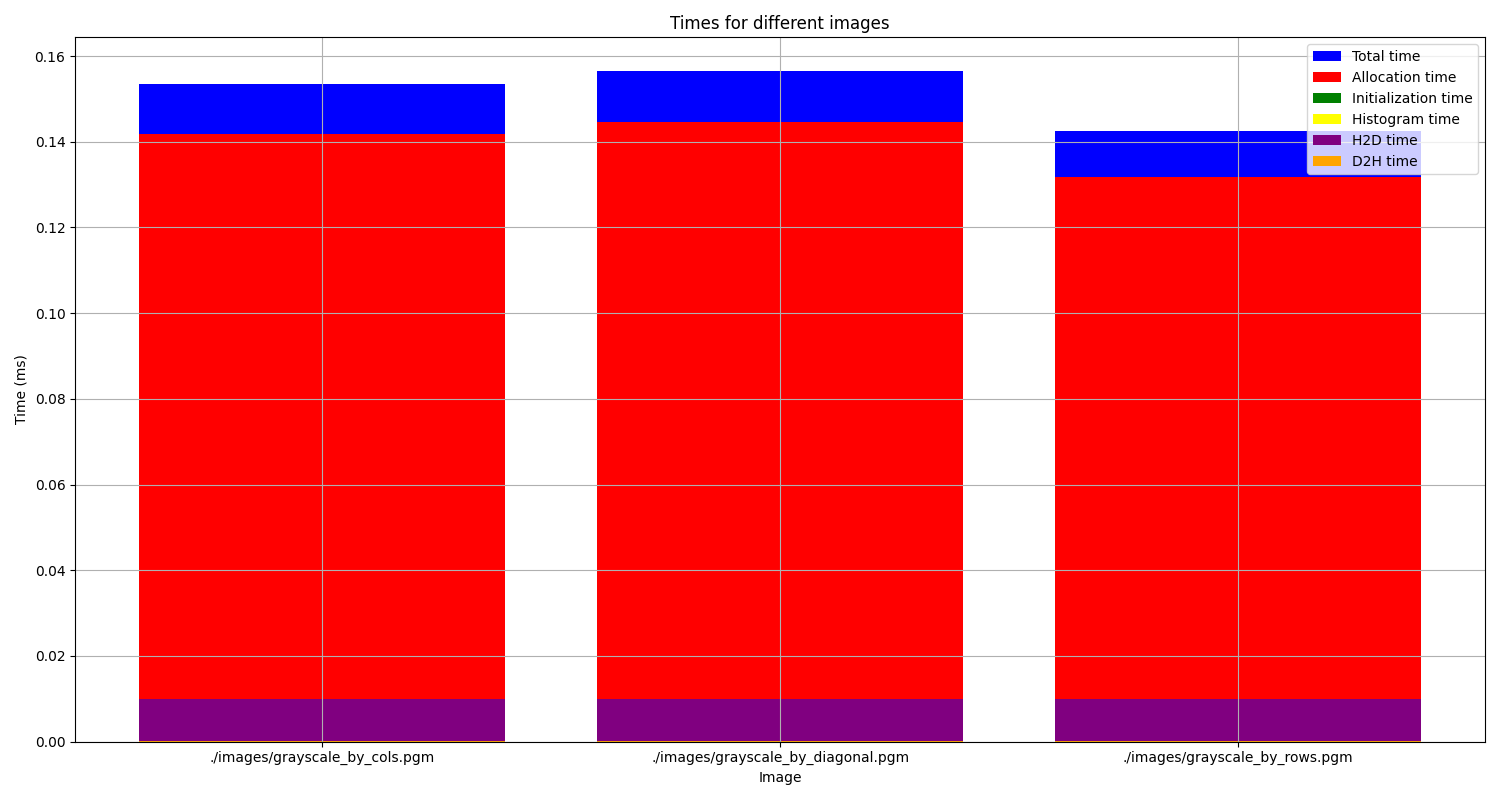
\includegraphics[width=0.88\textwidth]{images/conv2d_1/execution_times.png}
            }
            \caption{Tiempos de ejecución según imagen usando memoria global.}
            \label{fig:conv_execution_times_global}
        \end{figure}
        
        \begin{figure}[H]
            \centering
            \fbox{
                \includegraphics[width=0.88\textwidth]{images/conv2d_2/execution_times_npp.png}
            }
            \caption{Tiempos de ejecución según imagen usando NPP.}
            \label{fig:conv_execution_times_npp}
        \end{figure}

        En la implementación con memoria global (figura \ref{fig:conv_execution_times_global}), se observa una distribución temporal donde el componente dominante es el movimiento de datos \textit{host to device} de la imagen (segmento naranka), representando aproximadamente 0.10ms de los 0.28ms totales. El siguiente segmento con más relevancia es la alocación de memoria(0.5ms) para la imagen. En los tres casos se mantiene el mismo ratio.

        La implementación con la librería NPP (figura \ref{fig:conv_execution_times_npp}) muestra unos resultados peores, con un tiempo total casi del doble en algunos casos (60ms). En este caso sigue destacando el movimiento de datos \textit{host to device} (con un tiempo similar). La principal diferencia es el tiempo de cálculo del algoritmo de convolución, que llega a representar en dos de los casos 0.17ms aproximadamente. Destaca también como el algoritmo no muestra resultados constantes para las diferentes imágenes.

        En el primer caso, como el peso del algoritmo es mucho inferior, el tiempo total se ve determinado por los procesos de alocación de memoria y movimiento de datos, que se mantienen constantes al tratarse de fotos del mismo tamaño. Por otro lado, usando la librería no se optienen resultados tan óptimos para el algoritmo, como los conseguidos implementando el algoritmo con memoria global.


        Esta 
        
        

    \subsection{Tiempo de ejecución}

        La figuras \ref{fig:conv_mem_bloc} muestra los tiempos de ejecución para las diferentes fases del cálculo de la convolución en función del número de \textit{threads} por bloque, para la implementación con memoria global.

        \begin{figure}[H]
            \centering
            \fbox{
                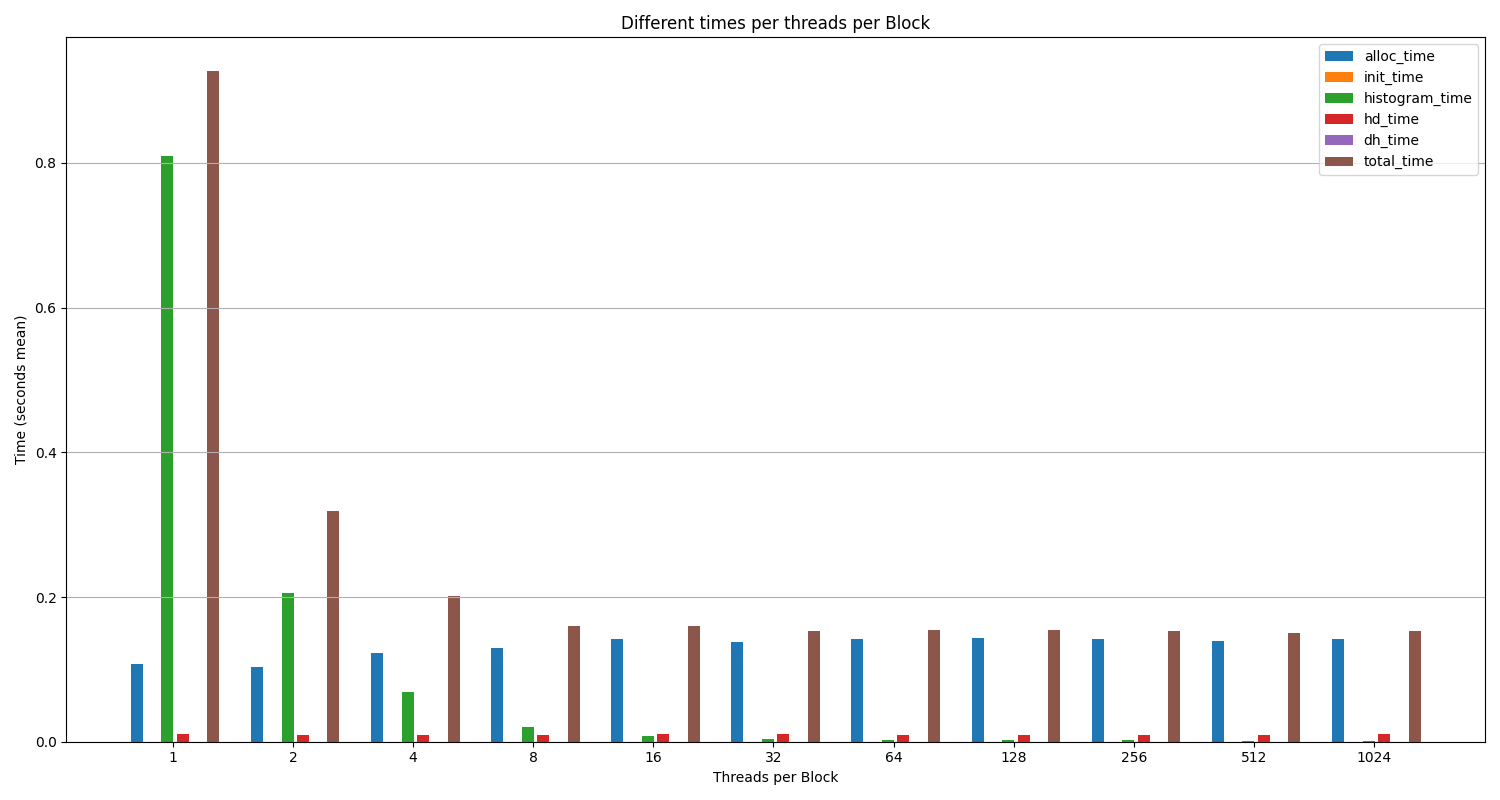
\includegraphics[width=0.9\textwidth]{images/conv2d_1/times_per_threadsPerBlock.png}
            }
            \caption{Tiempos de ejecución según el tamaño de bloque usando memoria global.}
            \label{fig:conv_mem_bloc}
        \end{figure}
        
        En la implementación con memoria global (figura \ref{fig:conv_mem_bloc}), se observa un comportamiento característico donde el tiempo de ejecución disminuye ligeramente en las configuraciones con menos hilos, para despues quedarse estancada. Si observamos la descomposición del tiempo global, vemos como el tiempo de reservar memoria y de mover los datos se mantiene estático para toda la muestra, y únicamente disminuye el tiempo de cálculo de la convolución.

        Este comportamiento puede asociarse a que se4 trabajan con imágenes de gran tamaño, y el operar con ellas en memoria (crearlas, moverlas, etc) supone un peso relativo muy grande en el tiempo total de ejecución. Este tipo de operaciones no se ven beneficiadas por el paralelismo de los hilos, lo que limita la mejora en el tiempo de ejecución.
        
       

    \subsection{Ocupancia}

        La figura \ref{fig:histogram_ioccupancy_per_threadsPerBlock} muestra cómo la ocupancia teórica de los multiprocesadores de la GPU (SM) varía en función del número de hilos por bloque, proporcionando información clave sobre la utilización de los recursos disponibles.

        \begin{figure}[H]
            \centering
            \fbox{
                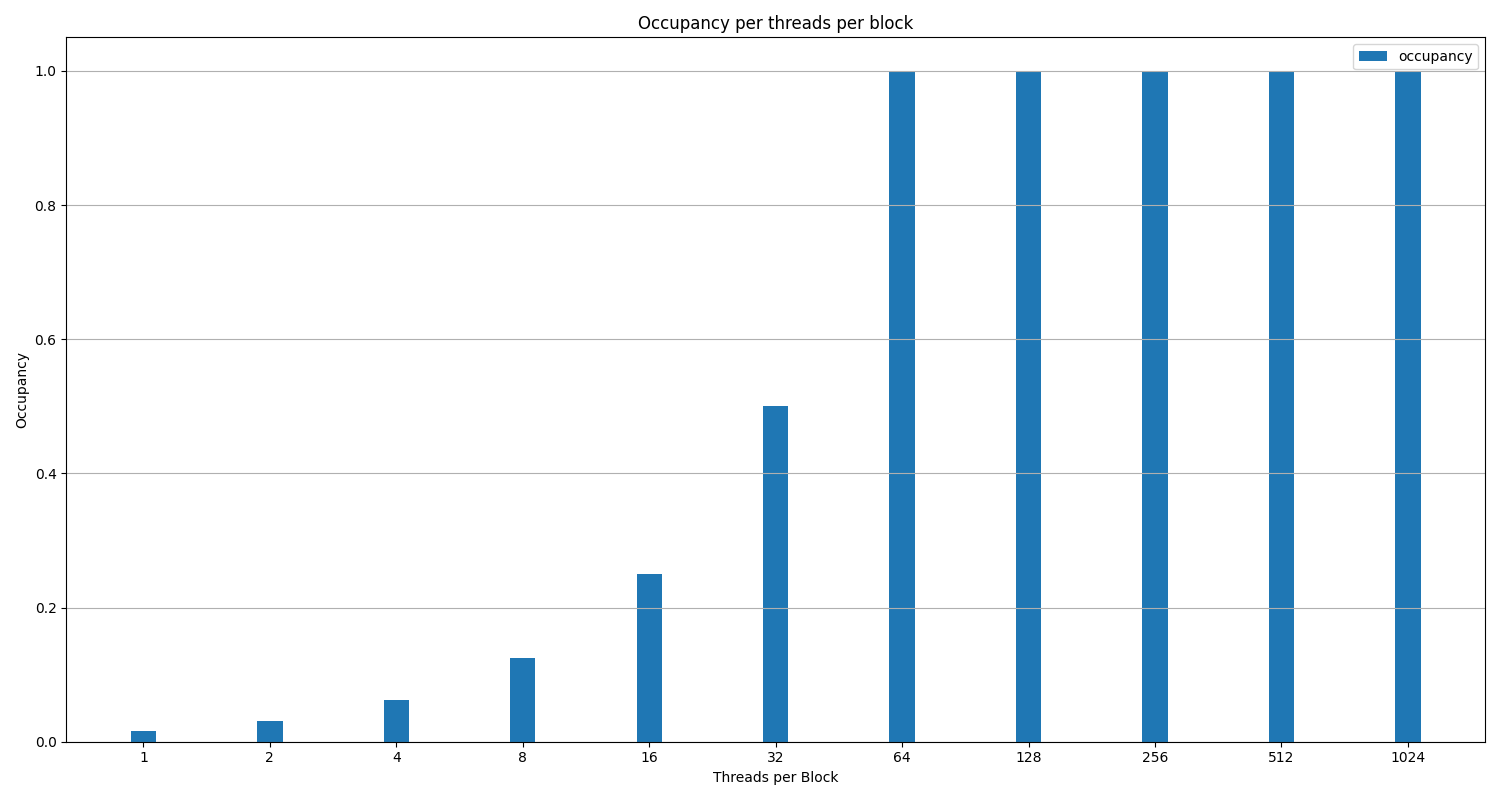
\includegraphics[width=0.9\textwidth]{images/conv2d_1/occupancy_per_threadsPerBlock.png}
            }
            \caption{Ocupancia según el tamaño de bloque.}
            \label{fig:conv2d_ioccupancy_per_threadsPerBlock}
        \end{figure}

        \begin{itemize}
        
            \item En configuraciones con un número reducido de hilos por bloque (1-32), la ocupancia es muy baja (inferior a 0.5), lo que explica el bajo rendimiento observado en estos casos. Una ocupancia reducida impide que el \textit{hardware} oculte de manera eficiente las latencias de acceso a memoria mediante el cambio de contexto entre \textit{warps}, resultando en una ejecución poco eficiente.
            
            \item Se observa un punto de inflexión importante en la configuración de 64 hilos por bloque, donde la ocupancia alcanza el valor máximo de 1.0 (100\%). Este valor se mantiene constante para configuraciones de 256, 512 y 1024 hilos por bloque. Sin embargo para configuraciones de 128 y 512 hilos la ocupancia se reduce ligeramente. Este comportamiento puede estar relacionado con la estructura de acceso del algoritmo de convolución.
        \end{itemize}
               
        
    \subsection{Matriz de isoeficiencia}

        La figura \ref{fig:convisoeficiency_global} muestra una  matriz de isoeficiencia que ofrece una perspectiva integral y multidimensional del rendimiento, considerando dos variables clave: el tamaño del problema en el eje horizontal, representado por las distintas imágenes examinadas y la cantidad de hilos por bloque en el eje vertical. Esta representación avanzada facilita la identificación de áreas con eficiencia similar en distintas configuraciones.

        \begin{figure}[H]
            \centering
            \fbox{
                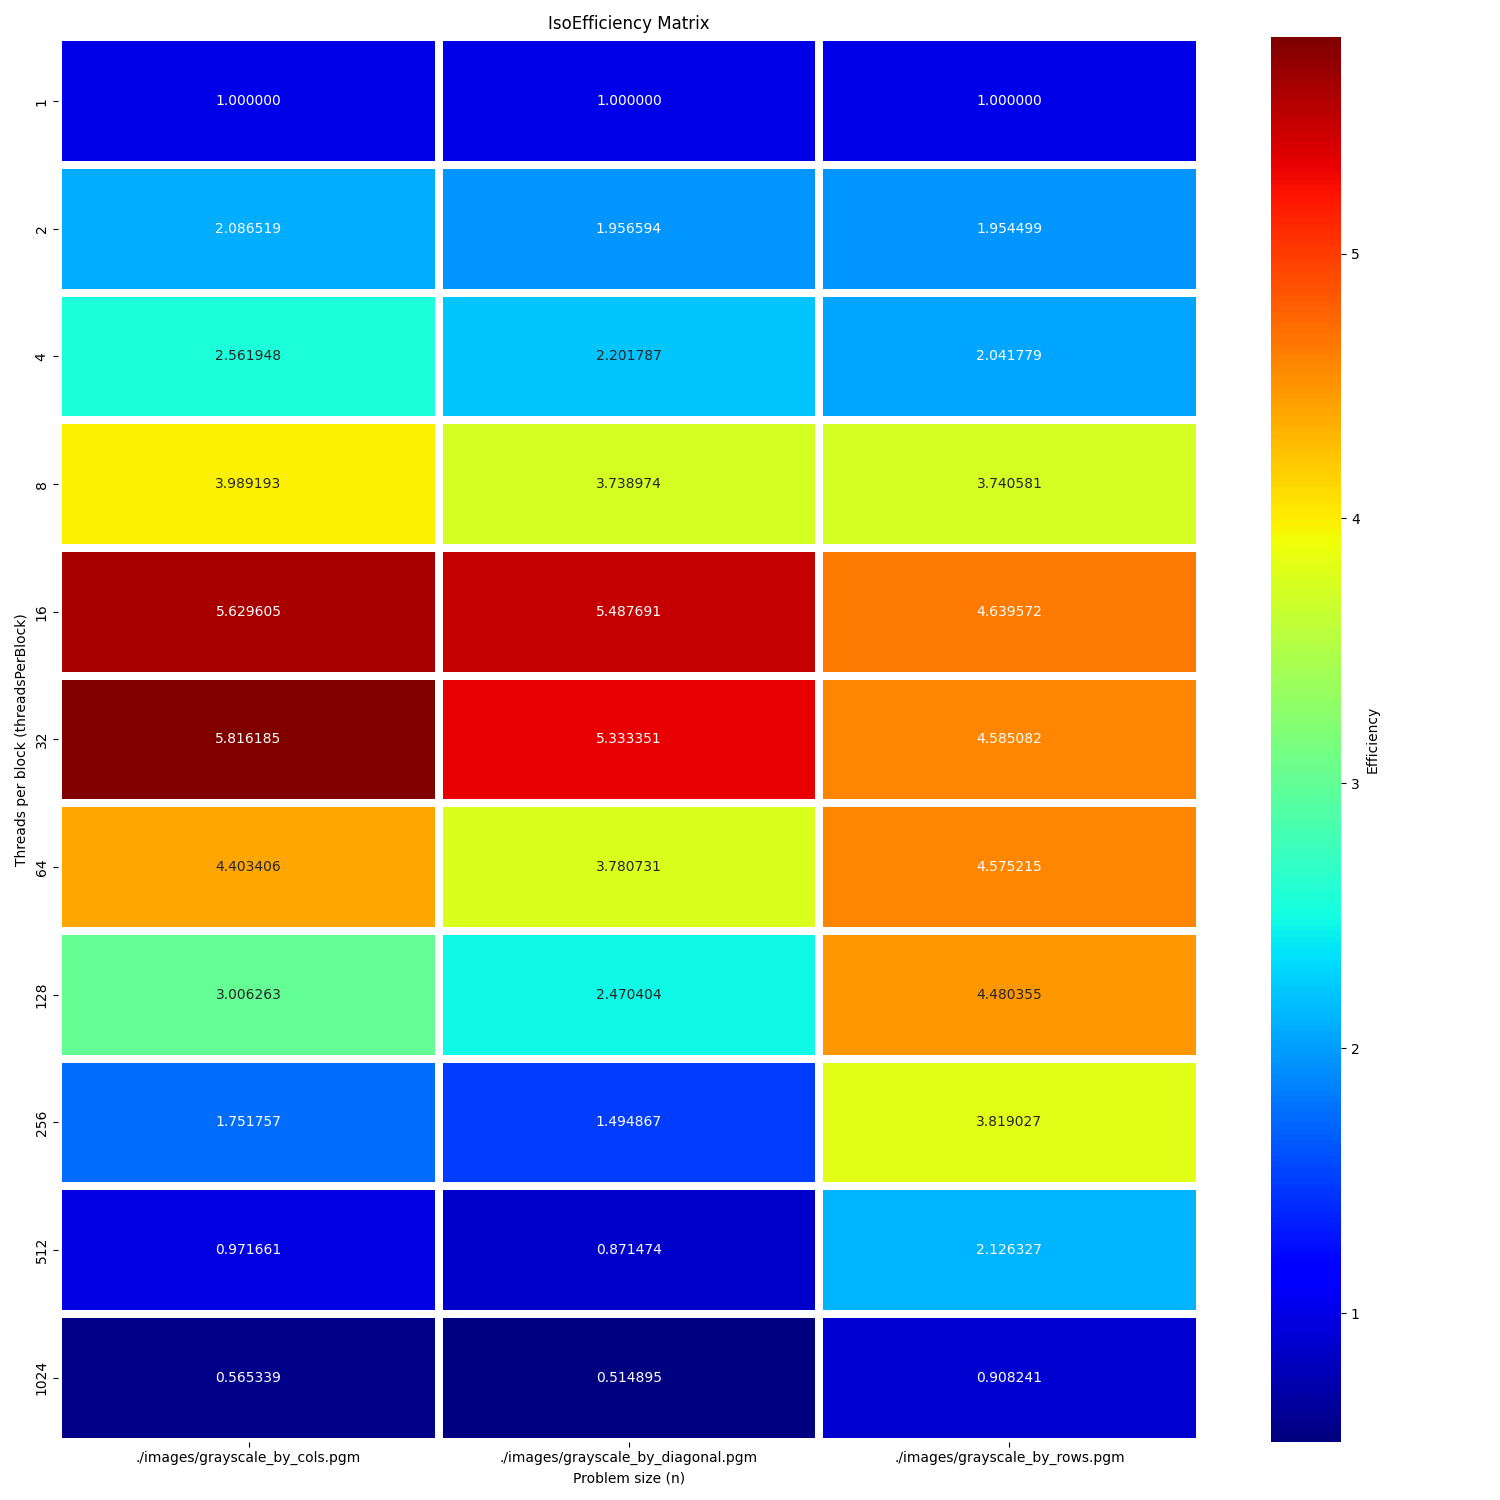
\includegraphics[width=0.9\textwidth]{images/conv2d_1/isoEfficiencyMatrix.png}
            }
            \caption{Matriz de isoeficiencia usando memoria global.}
            \label{fig:convisoeficiency_global}
        \end{figure}  

        En la matriz de isoeficiencia para la implementación con memoria global (figura \ref{fig:convisoeficiency_global}), se observa una tendencia donde la eficiencia decrece significativamente con configuraciones de hilos mayores. Los valores más altos de eficiencia (representados por colores rojo oscuro) se concentran en configuraciones con 1, 4 y 16 hilos por bloque. Esto sugiere que estas configuraciones logran un mejor aprovechamiento de los recursos de la GPU. También se observa baja eficiencia para configuraciones de hilos 2 y 8, lo que indica que estas configuraciones no logran explotar completamente el paralelismo disponible.

    \subsection{Métricas generales}

        \begin{table}[H]
            \centering
            \begin{adjustbox}{width=\textwidth, keepaspectratio}
                \begin{tabular}{rlrrrrrrr}
                    \toprule
                     threads &                          imagePath &  MaxTime &  RefTime &  Speedup &  Efficiency &  Quality &  SecuentialComputeSpeedup &  SecuentialTotalSpeedup \\
                    \midrule
                           1 &     ./images/grayscale\_by\_cols.pgm &     0.15 &     0.15 &     1.00 &        1.00 &     6.85 &                      8.95 &                    3.74 \\
                           2 &     ./images/grayscale\_by\_cols.pgm &     0.15 &     0.15 &     1.00 &        0.50 &     6.85 &                      8.95 &                    3.74 \\
                           4 &     ./images/grayscale\_by\_cols.pgm &     0.04 &     0.15 &     3.97 &        0.99 &    27.22 &                     35.56 &                    5.12 \\
                           8 &     ./images/grayscale\_by\_cols.pgm &     0.04 &     0.15 &     3.97 &        0.50 &    27.22 &                     35.56 &                    5.11 \\
                          16 &     ./images/grayscale\_by\_cols.pgm &     0.01 &     0.15 &    15.09 &        0.94 &   103.38 &                    135.06 &                    5.52 \\
                          32 &     ./images/grayscale\_by\_cols.pgm &     0.01 &     0.15 &    23.34 &        0.73 &   159.89 &                    208.88 &                    5.56 \\
                          64 &     ./images/grayscale\_by\_cols.pgm &     0.00 &     0.15 &    42.00 &        0.66 &   287.70 &                    375.85 &                    5.66 \\
                         128 &     ./images/grayscale\_by\_cols.pgm &     0.00 &     0.15 &    50.01 &        0.39 &   342.60 &                    447.58 &                    5.56 \\
                         256 &     ./images/grayscale\_by\_cols.pgm &     0.00 &     0.15 &    48.74 &        0.19 &   333.90 &                    436.20 &                    5.53 \\
                         512 &     ./images/grayscale\_by\_cols.pgm &     0.00 &     0.15 &    45.56 &        0.09 &   312.09 &                    407.71 &                    5.53 \\
                        1024 &     ./images/grayscale\_by\_cols.pgm &     0.00 &     0.15 &    39.12 &        0.04 &   267.99 &                    350.11 &                    5.63 \\
                           1 & ./images/grayscale\_by\_diagonal.pgm &     0.15 &     0.15 &     1.00 &        1.00 &     6.85 &                      8.95 &                    3.80 \\
                           2 & ./images/grayscale\_by\_diagonal.pgm &     0.15 &     0.15 &     1.00 &        0.50 &     6.85 &                      8.95 &                    3.78 \\
                           4 & ./images/grayscale\_by\_diagonal.pgm &     0.04 &     0.15 &     3.97 &        0.99 &    27.22 &                     35.56 &                    5.01 \\
                           8 & ./images/grayscale\_by\_diagonal.pgm &     0.04 &     0.15 &     3.97 &        0.50 &    27.22 &                     35.56 &                    5.08 \\
                          16 & ./images/grayscale\_by\_diagonal.pgm &     0.01 &     0.15 &    15.09 &        0.94 &   103.37 &                    135.04 &                    5.43 \\
                          32 & ./images/grayscale\_by\_diagonal.pgm &     0.01 &     0.15 &    23.34 &        0.73 &   159.89 &                    208.87 &                    5.55 \\
                          64 & ./images/grayscale\_by\_diagonal.pgm &     0.00 &     0.15 &    42.02 &        0.66 &   287.89 &                    376.10 &                    5.46 \\
                         128 & ./images/grayscale\_by\_diagonal.pgm &     0.00 &     0.15 &    50.00 &        0.39 &   342.51 &                    447.46 &                    5.62 \\
                         256 & ./images/grayscale\_by\_diagonal.pgm &     0.00 &     0.15 &    48.75 &        0.19 &   333.95 &                    436.27 &                    5.65 \\
                         512 & ./images/grayscale\_by\_diagonal.pgm &     0.00 &     0.15 &    45.55 &        0.09 &   312.03 &                    407.63 &                    5.58 \\
                        1024 & ./images/grayscale\_by\_diagonal.pgm &     0.00 &     0.15 &    39.12 &        0.04 &   268.03 &                    350.15 &                    5.60 \\
                           1 &     ./images/grayscale\_by\_rows.pgm &     0.15 &     0.15 &     1.00 &        1.00 &     6.85 &                      8.95 &                    3.72 \\
                           2 &     ./images/grayscale\_by\_rows.pgm &     0.15 &     0.15 &     1.00 &        0.50 &     6.85 &                      8.95 &                    3.79 \\
                           4 &     ./images/grayscale\_by\_rows.pgm &     0.04 &     0.15 &     3.97 &        0.99 &    27.22 &                     35.56 &                    5.08 \\
                           8 &     ./images/grayscale\_by\_rows.pgm &     0.04 &     0.15 &     3.97 &        0.50 &    27.22 &                     35.56 &                    5.05 \\
                          16 &     ./images/grayscale\_by\_rows.pgm &     0.01 &     0.15 &    15.09 &        0.94 &   103.38 &                    135.05 &                    5.48 \\
                          32 &     ./images/grayscale\_by\_rows.pgm &     0.01 &     0.15 &    23.34 &        0.73 &   159.88 &                    208.87 &                    5.57 \\
                          64 &     ./images/grayscale\_by\_rows.pgm &     0.00 &     0.15 &    42.02 &        0.66 &   287.85 &                    376.05 &                    5.57 \\
                         128 &     ./images/grayscale\_by\_rows.pgm &     0.00 &     0.15 &    49.98 &        0.39 &   342.40 &                    447.31 &                    5.55 \\
                         256 &     ./images/grayscale\_by\_rows.pgm &     0.00 &     0.15 &    48.75 &        0.19 &   333.95 &                    436.28 &                    5.57 \\
                         512 &     ./images/grayscale\_by\_rows.pgm &     0.00 &     0.15 &    45.57 &        0.09 &   312.16 &                    407.81 &                    5.61 \\
                        1024 &     ./images/grayscale\_by\_rows.pgm &     0.00 &     0.15 &    39.11 &        0.04 &   267.95 &                    350.05 &                    5.59 \\
                    \bottomrule
                    \end{tabular}
                    
            \end{adjustbox}
            \caption{Métricas generales usando memoria global.}
            \label{tab:conv2d}
        \end{table}

        \begin{table}[H]
            \centering
            \begin{adjustbox}{width=\textwidth, keepaspectratio}
                \begin{tabular}{lrrrrrr}
                    \toprule
                                             imagePath &  MaxTime &  RefTime &  Speedup &  Quality &  SecuentialComputeSpeedup &  SecuentialTotalSpeedup \\
                    \midrule
                        ./images/grayscale\_by\_cols.pgm &     1.07 &     1.07 &     1.00 &     0.93 &                      1.22 &                    1.23 \\
                    ./images/grayscale\_by\_diagonal.pgm &     0.29 &     0.29 &     1.00 &     3.39 &                      4.43 &                    3.02 \\
                        ./images/grayscale\_by\_rows.pgm &     0.29 &     0.29 &     1.00 &     3.43 &                      4.48 &                    3.04 \\
                    \bottomrule
                    \end{tabular}
                    
            \end{adjustbox}
            \caption{Métricas generales usando NPPI.}
            \label{tab:npp}
        \end{table} 
